\documentclass[main.tex]{subfiles}

\begin{document}


The \index{IceCube Neutrino Observatory} is described at length in Ref.~\cite{Aartsen_2017}. Briefly, the detector is a cubic-kilometer Cherenkov neutrino observatory one and half kilometers deep in the Antarctic ice~\cite{Aartsen_2017}.
There, 5160 photo-multiplier tubes encased within glass pressure vessels, or ``Digital Optical Modules'' (DOMs)~\cite{ABBASI2009294} detect Cherenkov emission from charged particles traversing the ice.
The DOMs are arranged vertically with a seventeen meter spacing into seventy-nine strings, which themselves are aligned into a hexagonal lattice with a 125 meter spacing. 
An additional, more densely instrumented sub-detector called DeepCore exists towards the bottom-center of the main detector~\cite{ABBASI2012615}.
The observatory has been running for over a decade and has accumulated large numbers of $\nu_{\mu}$ CC interactions which make depositions of light that make long signatures in the detector called tracks; and neutral current, electron neutrino, and tau neutrino events which deposit light in blob-like shapes called cascades. These event topologies are elaborated upon in Section. %~\ref{sec:depo}.

\section{The Ice}
As discussed in Ref~\cite{journal_glaciology_2013}, the Antarctic ice of IceCube is a rapidly-moving\footnote{several meters per annum} glacier formed over hundreds of thousands of years of compacted snowfall. 
The first few hundred meters, known as the \textit{firn} layer, is an opaque layer of recent snow. 
At greater depths the combined weight of the snow above compresses the firn snow into ice characterized by short scattering lengths dominatd by trapped bubbles of air.
Eventually the pressures reach extreme enough levels such that a new phase of ice takes shape; the trapped air is forced into a new chrystaline structure within the ice. 
The resulting, \textit{clathrate} ice boasts good optical properties, where the optical defects are characterized instead by microscopic grains of dust. \index{ice!bulk}

The properties were studied during the deployment of IceCube using a dust logger, with which measurements were taken in six of the eighty six bore holes dug during the IceCube deployment. 
It was a long ruggedized device with a fan-shaped 404nm diode laster that would probe 60 degrees of the horizon in each pass, and a downward looking PMT at the bottom of the dust logger measured the intensity of back-scattered light. 
A diagram of the dust logger is shown in Figure~\ref{fig:dustlog}, and the resulting measurements are shown in Figure~\ref{fig:icetilt}.

\begin{figure}  
    \centering
    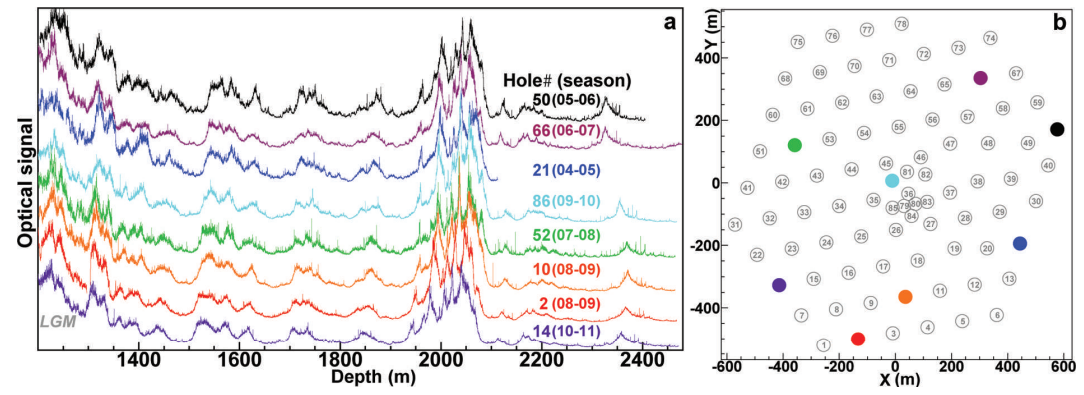
\includegraphics[width=0.8\linewidth]{figures/tilt.png}
    \caption{On the right we show which of the eighty six boreholes dustlogger data was taken, and on the left we show the intensity of the back-scatterd light as measured at each of the sampled holes as a function of depth.}\label{fig:icetilt}
\end{figure}


\begin{figure}
    \centering
    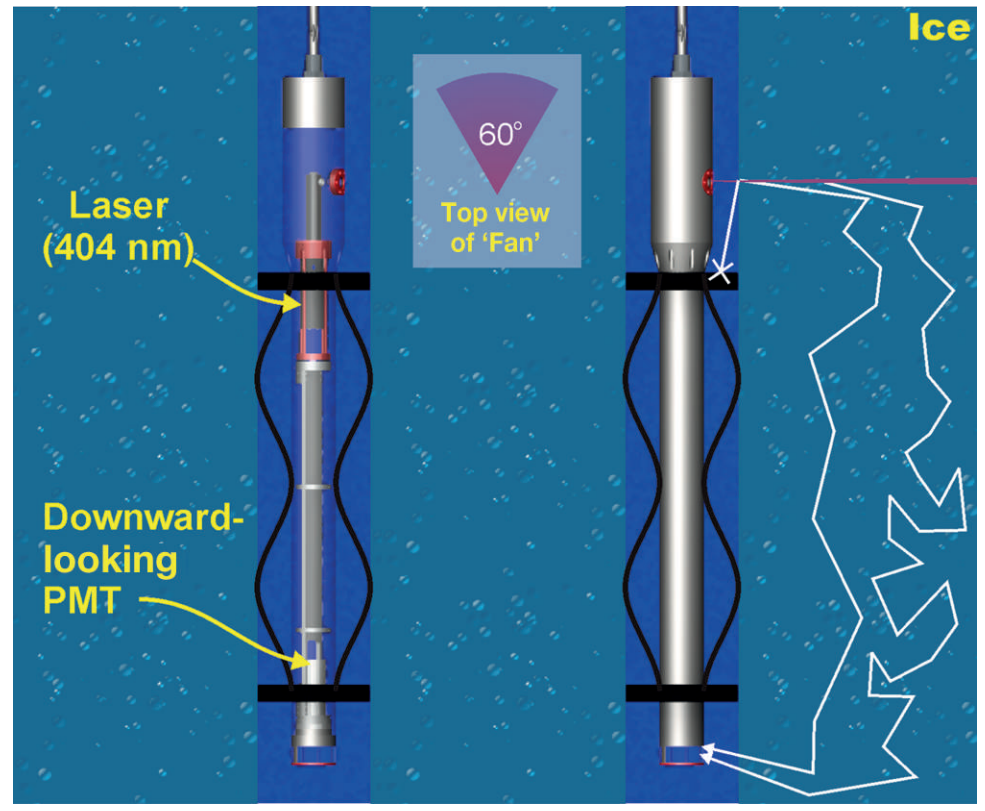
\includegraphics[width=0.6\linewidth]{figures/dustlog.png}
    \caption{A diagram of the IceCube dust logger.}\label{fig:dustlog}
\end{figure}

What we found was that the ice of IceCube is not uniform as a function of depth.
As the glacier around the present day location of IceCube moved over the eons, the pressures of the ice over the hard bedrock warped and bent the ice.
Layers of ice originally formed flat and at the same point in time grow bent and warped as they were themselves burried under greater depths of ice. 
Since the ice of IceCube is composed of the deeper ice characterized by pollutants in the ice, layers formed at the same point in time tend to have similar ice optical properties. 
The result of this is that the layers of ice with similar optical properties are not flat layers, but twisted and ``tilted.''   \index{ice!tilt}


\begin{figure}  
    \centering
    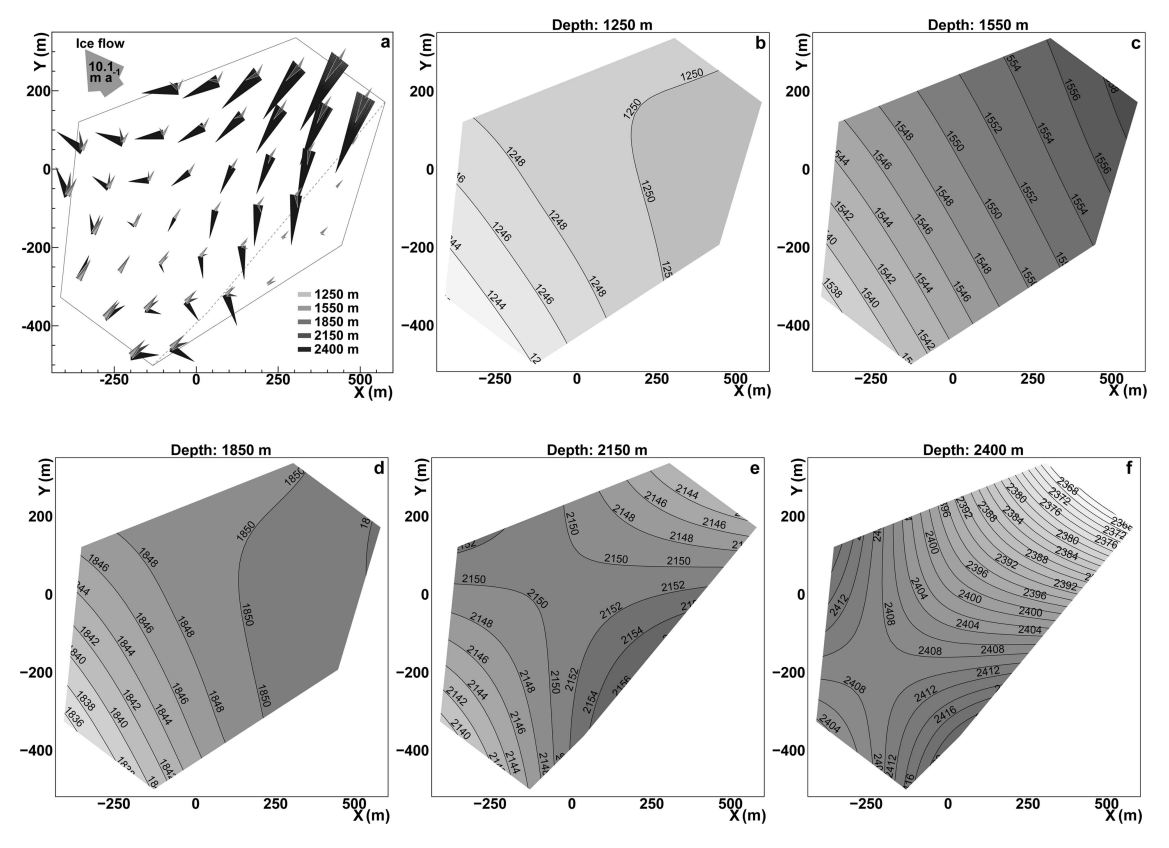
\includegraphics[width=0.8\linewidth]{figures/icecube_isochron.png}
    \caption{(a) shows the flow direction of the south pole glacier}\label{fig:isochron}
\end{figure}


Another complication arose during the deployment of IceCube. 
A hot-water drill was used to prepare the bore holes in which the strings of DOMs were inserted. 
After the DOM installation, the water in the bore holes refroze, but in an imperfect way.
The refrozen ice was exceptionally bubbly, yielding a much shorter scattering length in this region.
This ice is known as the \index{ice!hole ice} hole ice. 

Ice anisotropy! 

\section{Event topologies}

Large-volume neutrino telescopes typically are sensitive in the TeV to PeV energies; here, Deep-Inelastic Scattering (DIS)~\cite{gandhineutrinos} and the recently-observed~\cite{IceCube:2021rpz} Glashow-Resonance~\cite{PhysRev.118.316} interactions dominate. 
The detected neutrino interaction events fall into two morphological categories: tracks and cascades.

Charged-current (CC) $\nu_{\mu}$ DIS events result in muons at energies where radiative processes dominate energy loss rates.
As a result, energy losses are stochastically driven and the produced muons travel for kilometers. 
The results are threefold: muons are difficult to fully contain in neutrino telescopes, muon energies are poorly correlated with progenitor muon-neutrino energies, and muons' long travel-distance can allow for reconstructing their direction to within 1$^{\circ}$~\cite{trackaccuracy2017}. These events are called \textit{tracks}~\cite{icecube_energy_reco}.

All neutral-current (NC) DIS events result in a hadronic shower spreading around the interaction point and a secondary neutrino invisibly carrying away a proportion of the parent neutrino's energy. 
These events are often contained with a spherical topology. 
$\nu_{e}$-CC interactions develop similarly to neutral-current interactions, but repeated inverse Compton scattering of the produced electron initiates an electromagnetic shower superimposed over the hadronic shower. 
Thus, nearly all of the interacting neutrino's energy is observable as detectable light. 
These events are called \textit{cascades.} Such events tend to be well-contained permitting an efficient energy reconstruction, although suffer from poor angular reconstruction~\cite{icecube_energy_reco}. 

The evolution of a $\nu_{\tau}$-CC interaction is highly dependent on the energies involved. A tau is produced simultaneously as a hadronic cascade propagates around the interaction point, and then the tau decays. 
Due to their large mass, taus have a short lifetime and a decay length of $\sim 50$ m per PeV of tau energy~\cite{abbasi2020measurement}. 
From the tau branching ratios~\cite{PhysRevD.98.030001}, 17.37\% of the charged tau decays evolve as muon tracks, while the remainder of the decays evolve as electromagnetic or hadronic cascades. Only at neutrino energies above 60 TeV do $\nu_{\tau}$-CC interactions yield events with distinguishable primary and secondary cascades~\cite{abbasi2020measurement}.

Several distinct event samples have been developed to study these different types of events in IceCube. The High-Energy Starting Events sample~\cite{2021hese}, for example, was developed to study both taus and high-energy neutrinos likely astrophysical in origin. There exist other events samples optimized for higher event rates at lower energies, such as the Medium-Energy Starting Events~\cite{PhysRevDoverone}, and the five-year inelasticity sample~\cite{inelasticity2019}. There are also samples optimized for muon purity, such as the eight-year atmospheric muon sample~\cite{Aartsen_2020_prd} and others optimized for accurate energy resolution such as the six-years cascade sample~\cite{sixyrscascade}. This work will consider the cascade event selection described in~\cite{2018PhDT17N} and the track event selection previously used in IceCube sterile neutrino searches~\cite{PhysRevLett.117.071801}.

\end{document}